\documentclass[10pt]{article}
\usepackage[a4paper,margin=1.6cm,top=1.3cm,bottom=1.3cm]{geometry}
\usepackage[T1]{fontenc}
\usepackage{lmodern}
\usepackage{microtype}
\usepackage{booktabs}
\usepackage{graphicx}
\usepackage{enumitem}
\usepackage{xcolor}
\usepackage[colorlinks=true,linkcolor=black,citecolor=black,urlcolor=blue]{hyperref}
\setlist{nosep,leftmargin=1.2em,topsep=1pt}
\setlength{\parindent}{0pt}
\setlength{\parskip}{3pt}
\pagestyle{empty}
\newcommand{\head}[1]{\par\smallskip{\large\bfseries #1}\par}
\newcommand{\sect}[1]{\par\smallskip{\bfseries\color{black!80} #1}\par}

\begin{document}
\head{Idea 4 PoC --- Whose earnings expectations do Chinese prices reflect?}
\textit{Proof of concept, October 2026. Code: \texttt{idea04\_whose\_expectations/run.py}.}

\sect{Question and design}
Do A-share prices treat earnings as surprising relative to a naive seasonal random walk (SRW), or relative to a
better, look-ahead-free forecast? The SRW surprise splits exactly into two parts. The first is the part that the
out-of-sample XGBoost model predicted before the announcement,
$PRED=(\hat{E}^{XGB}-\hat{E}^{SRW})/\sigma$. The second is the XGBoost surprise $SUE^{XGB}=(E-\hat{E}^{XGB})/\sigma$.
Both share the same scale $\sigma$, the SD of the firm's last eight SRW errors. If the market used naive
expectations, $PRED$ would move announcement returns as much as $SUE^{XGB}$ does (as in Bernard and Thomas, 1990).
If it used ML-quality expectations, $PRED$ would already be priced. Sample: 104{,}487 quarterly announcements,
2005--2020, 158 announcement months. Returns are adjusted with size-decile benchmarks. Estimation is
Fama--MacBeth by announcement month with Newey--West $t$-statistics.

\begin{center}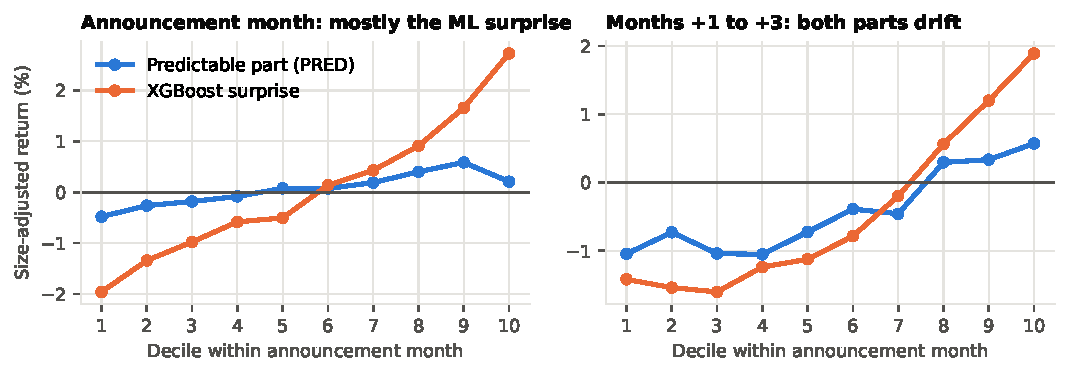
\includegraphics[width=0.97\textwidth]{results/fig_main.pdf}\end{center}

\begin{center}\small
\begin{tabular}{lccc}
\toprule
Window (size-adjusted return) & Months $-2,-1$ & Announcement month & Months $+1$ to $+3$\\
\midrule
$PRED$ (predicted before announcement) & 1.08 (6.6) & 0.11 (0.9) & 0.60 (3.5)\\
$SUE^{XGB}$ (XGBoost surprise) & 0.97 (8.4) & 0.73 (9.7) & 0.52 (4.7)\\
\midrule
Ratio $PRED/SUE^{XGB}$ & 1.11 & 0.15 & 1.16\\
\bottomrule
\end{tabular}\\[2pt]
{\footnotesize Coefficients in \% return per unit of SUE ($t$-statistics). Announcement-month test of equality:
$t=-5.8$. With size, B/M, momentum and turnover controls, the announcement-month $PRED$ coefficient is 0.18 ($t=1.4$).}
\end{center}

\sect{Findings}
\begin{itemize}
\item \textbf{At the announcement, prices react to the ML surprise, not the predictable part.} The announcement-month
  response to $PRED$ is only 15\% of the response to $SUE^{XGB}$ and is statistically zero. The market does not act
  as if it used the naive SRW benchmark. The two surprises explain about the same share of returns ($R^2$ 2.0\%
  against 1.9\%).
\item \textbf{The predictable part is priced slowly, not at the announcement.} $PRED$ predicts returns in the two
  months \emph{before} the announcement, consistent with leakage and China's mandatory preannouncements. It also
  predicts returns in the three months \emph{after}, by as much as the true surprise does. Information that a
  statistical model had in advance is still being incorporated one to three months after it is disclosed.
\item \textbf{Analyst coverage behaves unexpectedly.} The announcement-month reaction to $PRED$ is zero for firms
  without analyst coverage, but positive for covered firms (0.42, $t=2.9$). A possible reason is that analysts'
  forecasts themselves lag the statistical forecast.
\item \textbf{A tradable version is weak.} Sorting announcers at the start of the month on $PRED$, using only
  inputs public before the month, earns a Q5$-$Q1 spread of 0.45\%/month ($t=1.6$; CH-4 $\alpha=0.45\%$, $t=1.5$).
\end{itemize}

\sect{Assessment and next steps}
The headline is not ``naive expectations''. It is a timing result: predictable earnings information is priced
gradually around the announcement rather than at it. That is a sharper and more novel framing. Next steps:
(i) use daily returns to separate the preannouncement, announcement-day and drift windows; (ii) merge
preannouncement records to test whether the pre-announcement $PRED$ effect is the preannouncement channel; (iii)
add an analyst quarterly surprise, which needs I/B/E/S quarterly detail rather than the 12-month blend in the
panel; (iv) run placebo tests with shuffled $PRED$.
\end{document}
